% Options for packages loaded elsewhere
\PassOptionsToPackage{unicode}{hyperref}
\PassOptionsToPackage{hyphens}{url}
\PassOptionsToPackage{dvipsnames,svgnames,x11names}{xcolor}
%
\documentclass[
  number,
  preprint,
  3p,
  onecolumn]{elsarticle}

\usepackage{amsmath,amssymb}
\usepackage{iftex}
\ifPDFTeX
  \usepackage[T1]{fontenc}
  \usepackage[utf8]{inputenc}
  \usepackage{textcomp} % provide euro and other symbols
\else % if luatex or xetex
  \usepackage{unicode-math}
  \defaultfontfeatures{Scale=MatchLowercase}
  \defaultfontfeatures[\rmfamily]{Ligatures=TeX,Scale=1}
\fi
\usepackage{lmodern}
\ifPDFTeX\else  
    % xetex/luatex font selection
\fi
% Use upquote if available, for straight quotes in verbatim environments
\IfFileExists{upquote.sty}{\usepackage{upquote}}{}
\IfFileExists{microtype.sty}{% use microtype if available
  \usepackage[]{microtype}
  \UseMicrotypeSet[protrusion]{basicmath} % disable protrusion for tt fonts
}{}
\makeatletter
\@ifundefined{KOMAClassName}{% if non-KOMA class
  \IfFileExists{parskip.sty}{%
    \usepackage{parskip}
  }{% else
    \setlength{\parindent}{0pt}
    \setlength{\parskip}{6pt plus 2pt minus 1pt}}
}{% if KOMA class
  \KOMAoptions{parskip=half}}
\makeatother
\usepackage{xcolor}
\setlength{\emergencystretch}{3em} % prevent overfull lines
\setcounter{secnumdepth}{5}
% Make \paragraph and \subparagraph free-standing
\makeatletter
\ifx\paragraph\undefined\else
  \let\oldparagraph\paragraph
  \renewcommand{\paragraph}{
    \@ifstar
      \xxxParagraphStar
      \xxxParagraphNoStar
  }
  \newcommand{\xxxParagraphStar}[1]{\oldparagraph*{#1}\mbox{}}
  \newcommand{\xxxParagraphNoStar}[1]{\oldparagraph{#1}\mbox{}}
\fi
\ifx\subparagraph\undefined\else
  \let\oldsubparagraph\subparagraph
  \renewcommand{\subparagraph}{
    \@ifstar
      \xxxSubParagraphStar
      \xxxSubParagraphNoStar
  }
  \newcommand{\xxxSubParagraphStar}[1]{\oldsubparagraph*{#1}\mbox{}}
  \newcommand{\xxxSubParagraphNoStar}[1]{\oldsubparagraph{#1}\mbox{}}
\fi
\makeatother


\providecommand{\tightlist}{%
  \setlength{\itemsep}{0pt}\setlength{\parskip}{0pt}}\usepackage{longtable,booktabs,array}
\usepackage{calc} % for calculating minipage widths
% Correct order of tables after \paragraph or \subparagraph
\usepackage{etoolbox}
\makeatletter
\patchcmd\longtable{\par}{\if@noskipsec\mbox{}\fi\par}{}{}
\makeatother
% Allow footnotes in longtable head/foot
\IfFileExists{footnotehyper.sty}{\usepackage{footnotehyper}}{\usepackage{footnote}}
\makesavenoteenv{longtable}
\usepackage{graphicx}
\makeatletter
\def\maxwidth{\ifdim\Gin@nat@width>\linewidth\linewidth\else\Gin@nat@width\fi}
\def\maxheight{\ifdim\Gin@nat@height>\textheight\textheight\else\Gin@nat@height\fi}
\makeatother
% Scale images if necessary, so that they will not overflow the page
% margins by default, and it is still possible to overwrite the defaults
% using explicit options in \includegraphics[width, height, ...]{}
\setkeys{Gin}{width=\maxwidth,height=\maxheight,keepaspectratio}
% Set default figure placement to htbp
\makeatletter
\def\fps@figure{htbp}
\makeatother

\makeatletter
\@ifpackageloaded{caption}{}{\usepackage{caption}}
\AtBeginDocument{%
\ifdefined\contentsname
  \renewcommand*\contentsname{Table of contents}
\else
  \newcommand\contentsname{Table of contents}
\fi
\ifdefined\listfigurename
  \renewcommand*\listfigurename{List of Figures}
\else
  \newcommand\listfigurename{List of Figures}
\fi
\ifdefined\listtablename
  \renewcommand*\listtablename{List of Tables}
\else
  \newcommand\listtablename{List of Tables}
\fi
\ifdefined\figurename
  \renewcommand*\figurename{Figure}
\else
  \newcommand\figurename{Figure}
\fi
\ifdefined\tablename
  \renewcommand*\tablename{Table}
\else
  \newcommand\tablename{Table}
\fi
}
\@ifpackageloaded{float}{}{\usepackage{float}}
\floatstyle{ruled}
\@ifundefined{c@chapter}{\newfloat{codelisting}{h}{lop}}{\newfloat{codelisting}{h}{lop}[chapter]}
\floatname{codelisting}{Listing}
\newcommand*\listoflistings{\listof{codelisting}{List of Listings}}
\makeatother
\makeatletter
\makeatother
\makeatletter
\@ifpackageloaded{caption}{}{\usepackage{caption}}
\@ifpackageloaded{subcaption}{}{\usepackage{subcaption}}
\makeatother
\journal{Journal Name}

\ifLuaTeX
  \usepackage{selnolig}  % disable illegal ligatures
\fi
\usepackage[]{natbib}
\bibliographystyle{elsarticle-num}
\nocite{*}
\usepackage{bookmark}

\IfFileExists{xurl.sty}{\usepackage{xurl}}{} % add URL line breaks if available
\urlstyle{same} % disable monospaced font for URLs
\hypersetup{
  pdftitle={Un estudio sobre los retornos del mercado de renta fija dominicano utilizando basados en modelos AR-GARCH},
  pdfauthor={Ian Contreras},
  pdfkeywords={Mercado de renta fija, Deuda pública, Modelos AR-GARCH},
  colorlinks=true,
  linkcolor={blue},
  filecolor={Maroon},
  citecolor={Blue},
  urlcolor={Blue},
  pdfcreator={LaTeX via pandoc}}


\setlength{\parindent}{6pt}
\begin{document}

\begin{frontmatter}
\title{Un estudio sobre los retornos del mercado de renta fija
dominicano utilizando basados en modelos AR-GARCH \\\large{Trabajo final
de tópicos de econometría} }
\author[1]{Ian Contreras%
%
}
 \ead{1116048@intec.edu.do} 

\affiliation[1]{organization={INSTITUTO TECNOLÓGICO DE SANTO DOMINGO
(INTEC)},,postcodesep={}}

\cortext[cor1]{Corresponding author}

        
\begin{abstract}
Este estudio tiene como objetivo analizar los retornos y la volatilidad
del mercado de deuda pública dominicana mediante la aplicación de
modelos ARMA-GARCH. A través de estos modelos, se busca identificar
patrones en el comportamiento de los retornos y predecir su evolución
futura.
\end{abstract}





\begin{keyword}
    Mercado de renta fija \sep Deuda pública \sep 
    Modelos AR-GARCH
\end{keyword}
\end{frontmatter}
    

\phantomsection\label{importing-libraries}
\textsubscript{Source:
\href{https://iancont.github.io/fixed_income_garch/index.qmd.html}{Article
Notebook}}

\phantomsection\label{importing-data}
\textsubscript{Source:
\href{https://iancont.github.io/fixed_income_garch/index.qmd.html}{Article
Notebook}}

\section{Introducción}\label{introducciuxf3n}

El mercado de renta fija en la República Dominicana ha emergido como uno
de los sectores más importantes dentro de la economía, especialmente en
lo que respecta a la deuda pública, la cual juega un papel crucial en la
financiación de proyectos gubernamentales y el sostenimiento de la
política fiscal. En los últimos cincuenta años, el país ha experimentado
un crecimiento económico significativo, consolidándose como una de las
economías más dinámicas de América Latina. Este crecimiento ha estado
acompañado por una mayor complejidad económica, lo que ha incrementado
la relevancia del mercado financiero dominicano, en particular el
mercado de deuda pública, que ha sido un activo clave para fondos de
pensiones y fondos de inversión.

Sin embargo, este mercado también presenta importantes desafíos,
especialmente en términos de baja liquidez en el mercado secundario y
episodios de alta volatilidad. Estos problemas dificultan la previsión
precisa de los movimientos del mercado y complican la toma de decisiones
estratégicas para los inversores. En este contexto, surge la necesidad
de utilizar herramientas econométricas que puedan capturar con mayor
precisión las dinámicas subyacentes de los retornos y la volatilidad del
mercado de deuda pública dominicano.

La \textbf{pregunta de investigación} que guía este estudio es: ¿Es
posible modelar adecuadamente los retornos y la volatilidad del mercado
de deuda pública dominicano mediante modelos ARIMA-GARCH?, y ¿Qué tan
efectivas son estas técnicas para predecir el comportamiento futuro del
mercado, especialmente durante periodos de alta volatilidad?

El \textbf{objetivo principal} de este estudio es aplicar modelos
ARMA-GARCH para analizar y predecir el comportamiento de los retornos
del índice de deuda pública IRP-GOBIX, considerando tanto la tendencia
como los patrones de volatilidad del mercado. A través de la estimación
de estos modelos, se busca identificar los principales factores que
afectan la dinámica de los retornos y proporcionar información valiosa
para los actores del mercado, facilitando una gestión más eficiente del
riesgo.

Además, este estudio pretende evaluar la \textbf{consistencia de los
modelos} y determinar si los modelos de volatilidad más sofisticados,
como el Zero-GARCH, ofrecen una mejor capacidad de predicción que los
modelos tradicionales basados únicamente en niveles y diferencias, como
el ARIMA. Un aspecto clave será analizar si el modelo GARCH captura
adecuadamente los choques bruscos y los episodios de volatilidad
extrema, o si suaviza excesivamente estos movimientos.

La \textbf{relevancia} de este estudio radica en la creciente
importancia del mercado de deuda pública dominicano, tanto para la
estabilidad financiera del país como para los inversores extranjeros que
buscan oportunidades de inversión en mercados emergentes. Comprender los
patrones de retorno y volatilidad es esencial para diseñar estrategias
de inversión que minimicen el riesgo y maximicen el rendimiento en un
entorno económico globalizado y altamente incierto.

\section{Metodología}\label{metodologuxeda}

El modelo ARIMA(p,d,q), donde AR(p) es el componente autorregresivo de
orden p, d denota el orden de la diferencia aplicada para transformar
una serie temporal no estacionaria en estacionaria, y MA(q) representa
el promedio móvil de orden q. La esencia del modelo ARIMA radica en la
combinación de la operación de diferenciación y el modelo ARMA.
Cualquier serie no estacionaria puede volverse estacionaria mediante una
diferenciación de orden adecuado, permitiendo así ajustar un modelo ARMA
a la serie transformada.

El modelo de promedio móvil autorregresivo ARMA(p,q) incluye tanto un
componente autorregresivo de orden p como uno de promedio móvil de orden
q, y se estructura de la siguiente forma:

\[
X_t = \phi_1 X_{t-1} + \phi_2 X_{t-2} + \dots + \phi_p X_{t-p} + \epsilon_t + \theta_1 \epsilon_{t-1} + \theta_2 \epsilon_{t-2} + \dots + \theta_q \epsilon_{t-q}
\] \{eq: arma\}

Estos modelos son adecuados solo para describir series temporales
suaves, mientras que en la práctica, a menudo se trabaja con series
temporales no suaves. Para estos casos, aplicar una o dos
diferenciaciones puede transformar los datos en series suaves.

Si no se cumple el supuesto de homogeneidad de la varianza, puede
ocurrir heterocedasticidad. Dado que los datos de la muestra son suaves,
en este documento se establece un modelo ARMA(p,q) para la serie de
rendimientos con el fin de describir las características de volatilidad
del índice GOBIX. Se realizan pruebas de efecto ARCH y se resuelve el
problema de la heterocedasticidad mediante un modelo GARCH.

El modelo GARCH extiende el modelo ARCH al considerar la autocorrelación
de orden p en la función de heterocedasticidad, lo que permite ajustar
de manera efectiva una función de heterocedasticidad con memoria a largo
plazo. El modelo GARCH se define de la siguiente manera:

\[
a_t = \sigma_t \epsilon_t, \quad \sigma_t^2 = \alpha_0 + \sum_{i=1}^{p} \alpha_i a_{t-i}^2 + \sum_{j=1}^{q} \beta_j \sigma_{t-j}^2
\] \{\#eq: garch\}

El modelo GARCH, propuesto por Bollerslev, atribuye la volatilidad
actual tanto a la volatilidad de momentos pasados como a los errores de
momentos pasados, lo que le permite explicar el fenómeno de agrupación
en la volatilidad de los rendimientos financieros.

\section{Datos}\label{datos}

\subsection{Fuente de datos}\label{fuente-de-datos}

Un Índice Financiero es una medida estadística que refleja el valor de
un conjunto de activos financieros agrupados de acuerdo con ciertos
criterios.Estos se utilizan como objetivo de rendimiento de portafolios,
referencias sobre las características retorno/riesgo de una clase de
activo y como referencia para productos anclados a índices.

En el mercado de renta fija de la República Dominicana, el único índice
público es el GOBIX, que representa la deuda gubernamental consolidada
en peso. Este índice está compuesto por títulos emitidos localmente por
el Banco Central y el Ministerio de Hacienda, y se publica en dos
modalidades: índice de precio limpio e índice de retorno-precio. Para
este estudio, se utilizará el índice de retorno precio
Section~\ref{sec-retorno-precio}, ya que aisla el componente de retorno
de mercado el cual es el objetivo de estudio.

El GOBIX se caracteriza por los siguientes criterios:

\begin{itemize}
\tightlist
\item
  \textbf{Elegibilidad}: Solo se incluyen títulos ``bullet'' emitidos en
  pesos dominicanos con al menos 60 días desde su emisión.
\item
  \textbf{Liquidez}: Los títulos se seleccionan en función del Índice de
  Bursatilidad publicado por la Proveedora de Precios, garantizando la
  inclusión de los instrumentos más negociados.
\item
  \textbf{Ponderación}: La ponderación se realiza por capitalización de
  mercado, lo que asegura que los títulos más relevantes tengan mayor
  peso en el índice.
\item
  \textbf{Rebalanceo}: Se efectúa un rebalanceo mensual para ajustar el
  índice según la disponibilidad de inversión en los bonos.
\item
  \textbf{Fuentes de información}: Los datos provienen de la Bolsa de
  Valores de la República Dominicana y la Proveedora de Precios.
\end{itemize}

\subsection{Índice de Retorno-Precio}\label{sec-retorno-precio}

El índice de retorno-precio es una metodología utilizada para calcular
el rendimiento de un índice de renta fija, centrándose exclusivamente en
las variaciones del precio limpio de los títulos, sin tener en cuenta
los intereses acumulados ni el pago de cupones durante el período de
cálculo. En el contexto del GOBIX, este índice refleja las fluctuaciones
en los precios de los bonos dominicanos debido a las variaciones en las
tasas de interés del mercado.

\textbf{Características del Índice de Retorno-Precio del GOBIX}:

\begin{itemize}
\item
  \textbf{Enfoque en el Precio Limpio}: El cálculo del índice se basa en
  el precio limpio de los bonos, excluyendo los intereses acumulados.
\item
  \textbf{Reflejo de la Volatilidad}: Este índice es un indicador del
  riesgo asociado a las fluctuaciones en las tasas de interés y su
  impacto en el capital invertido.
\item
  \textbf{Fórmula de Cálculo}:

  \[
  IRP_t = IRP_{m-1} \times (1 + RPI_t)
  \]

  Donde:

  \begin{itemize}
  \tightlist
  \item
    \(IRP_0 = 100\) es el valor base del índice en la fecha de inicio.
  \item
    \(IRP_t\) es el valor del índice en el día \(t\).
  \item
    \(IRP_{m-1}\) es el valor del índice en el último día hábil del mes
    anterior.
  \item
    \(RPI_t\) es el retorno-precio del índice en \(t\).
  \end{itemize}
\end{itemize}

El retorno-precio del índice (\(RPI_t\)) se calcula como la suma
ponderada del retorno-precio de cada bono (\(RPI_{i,t}\)), donde la
ponderación (\(\omega_i\)) se determina según la capitalización de
mercado de cada bono.

En este análisis, expresaremos la serie de retornos en puntos básicos
para evitar problemas de escalamiento de los datos y posibles
desbordamientos decimales (overflow decimal), que pueden ocurrir cuando
se manejan fluctuaciones muy pequeñas con alta precisión. Un punto
básico equivale a 0.01\% o 1/100 de un porcentaje. Este enfoque nos
permitirá manejar los datos con mayor estabilidad y evitar posibles
errores numéricos derivados del escalamiento inapropiado. No tiene
efectos estadísticos en las distribución.

\subsection{Selección de muestra de
entrenamiento/prueba}\label{sec-test-train}

Durante la pandemia, se experimentó uno de los ciclos de tasas de
interés más pronunciados de las últimas décadas. Este periodo presentó
características estructurales distintas en comparación con los ciclos
históricos previos. Para evitar sesgos en las estimaciones debido a la
alta volatilidad observada durante ese tiempo, evaluaremos únicamente la
serie de retornos entre el periodo 2014-2021, que se considera un ciclo
de tasas más regular.

La metodología empleada para dividir el conjunto de datos en muestras de
entrenamiento y prueba será el \textbf{Time Series Cross-Validator}. A
diferencia de la validación cruzada tradicional, que aleatoriza los
datos, esta técnica respeta el orden temporal, lo cual es crucial en el
análisis de series de tiempo.

En cada partición (k-ésimo split), la técnica funciona de la siguiente
manera:

\begin{itemize}
\tightlist
\item
  \textbf{Conjunto de Entrenamiento}: Incluye los primeros \emph{k}
  pliegues (folds).
\item
  \textbf{Conjunto de Prueba}: Incluye el pliegue \emph{(k+1)}.
\end{itemize}

\section{Análisis Exploratorio}\label{sec-eda}

El objetivo de este análisis exploratorio es examinar la serie de
retornos diarios del IRP-GOBIX para identificar patrones de volatilidad,
evaluar la distribución de los retornos, y explorar la autocorrelación
en los datos. Utilizando herramientas estadísticas como la distribución
de los retornos, el test de estacionariedad Dickey-Fuller, y los
gráficos de autocorrelación (ACF) y autocorrelación parcial (PACF), se
busca comprender la dinámica temporal de los retornos y validar la
aplicación de modelos ARMA-GARCH para capturar su comportamiento futuro.
Adicionalmente, se ajustarán diversas distribuciones teóricas, como la
distribución normal y la t de Student, para evaluar su capacidad de
describir las características empíricas de los datos.

\subsection{Histórico de retornos precio del mercado de deuda pública
dominicano}\label{sec-historico-retornos}

\begin{figure}[H]

\centering{

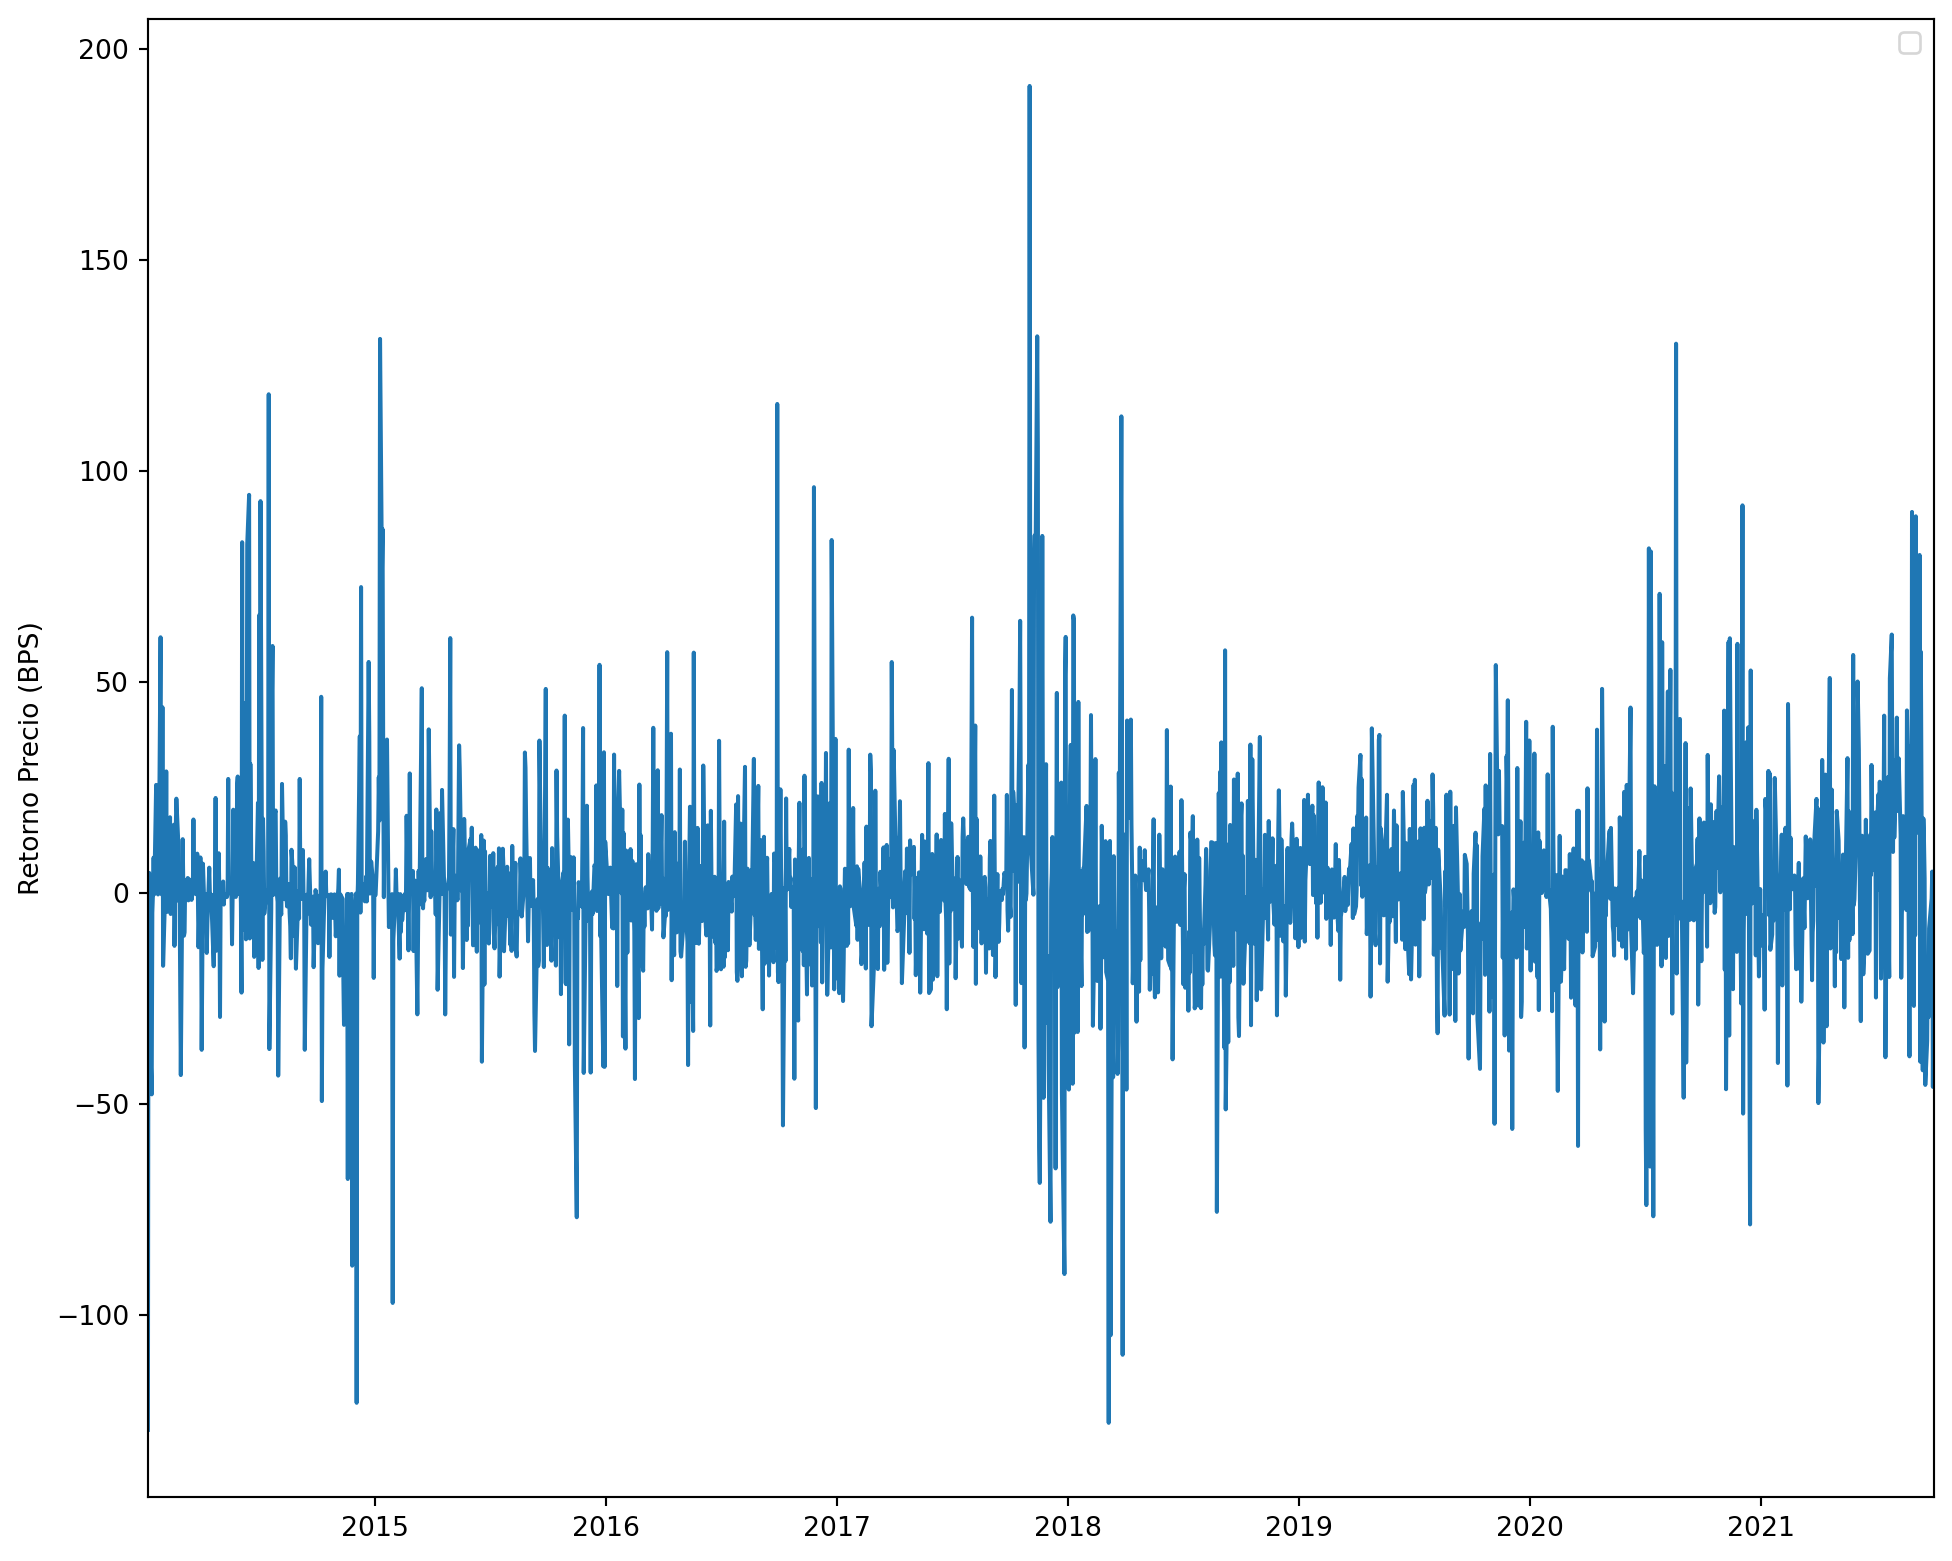
\includegraphics{index_files/figure-latex/notebooks-data-screening-fig-price-return-series-output-2.png}

}

\caption{\label{fig-price-return-series}Serie de retornos diarios
IRP-GOBIX.}

\end{figure}%

\textsubscript{Source:
\href{https://iancont.github.io/fixed_income_garch/index.qmd.html}{Article
Notebook}}

El análisis de la serie de retornos diarios del IRP-GOBIX revela un
comportamiento interesante, con periodos prolongados de baja volatilidad
seguidos por episodios de alta volatilidad. Entre 2015 y 2022, los
retornos se mantuvieron generalmente dentro de un rango de ±50 puntos
básicos, lo que indica una estabilidad relativa. Sin embargo, en
momentos clave, como el ciclo de tasas de 2018, la volatilidad se
incrementó drásticamente, alcanzando picos de hasta 200 puntos básicos.
Este patrón es característico del fenómeno conocido como
\textbf{``volatility clustering''}, donde periodos tranquilos son
seguidos por fases de mayor volatilidad. La naturaleza de estos picos
parece estar relacionada con factores externos, como cambios en las
tasas de interés y la incertidumbre macroeconómica global, lo que
subraya la importancia de emplear modelos ARMA-GARCH para capturar estas
dinámicas y prever comportamientos futuros en el mercado de deuda
pública dominicana.

\subsection{Análisis descriptivo de la
muestra}\label{sec-estadistica-descriptiva}

\textsubscript{Source:
\href{https://iancont.github.io/fixed_income_garch/index.qmd.html}{Article
Notebook}}

\begin{longtable}[]{@{}lllllllll@{}}
\toprule\noalign{}
& Observations & Mean & Median & Std. Dev & Skewness & Kurtosis &
Jarque-Bera & Prob. \\
\midrule\noalign{}
\endhead
\bottomrule\noalign{}
\endlastfoot
0 & 1941 & 1.353251 & -0.318044 & 23.502911 & 0.70527 & 7.587995 &
4789.532331 & 0.0 \\
\end{longtable}

Tabla de las estadísticas descriptiva de la serie de retornos

\textsubscript{Source:
\href{https://iancont.github.io/fixed_income_garch/index.qmd.html}{Article
Notebook}}

El análisis descriptivo de los retornos ofrece una perspectiva más
detallada sobre la distribución de la serie. Con un total de 1,941
observaciones, la \textbf{media} de los retornos es de \(1.353251\), lo
que indica un rendimiento promedio positivo. Sin embargo, la
\textbf{mediana} de \(-0.318044\) sugiere un leve sesgo hacia valores
negativos, lo que refleja que la mayoría de los retornos tienden a ser
ligeramente inferiores a la media. La \textbf{desviación estándar}, con
un valor de \(23.502911\), revela una amplia dispersión de los datos, lo
que confirma la presencia de una volatilidad significativa en los
rendimientos, muy superior al valor medio.

En cuanto a la \textbf{asimetría} (\(0.70527\)), se observa una ligera
inclinación hacia valores extremos positivos, lo que implica la
existencia de eventos fuera de lo común que afectan los rendimientos. La
\textbf{kurtosis} de \(7.587995\) indica una distribución
\textbf{leptocúrtica}, caracterizada por una alta concentración de
valores alrededor de la media y colas más gruesas que una distribución
normal, lo que es típico en datos financieros que presentan eventos
extremos. El \textbf{test de Jarque-Bera}, con un valor de
\(4,789.532331\), confirma que la serie no sigue una distribución
normal, validando la presencia de asimetría y colas pesadas en los
datos. Estos resultados resaltan la necesidad de emplear modelos que
puedan capturar adecuadamente estos comportamientos no lineales,
esenciales para el análisis del mercado.

\subsection{Análisis de la distribución de los
retornos}\label{sec-distribucion-retornos}

\begin{figure}[H]

\centering{

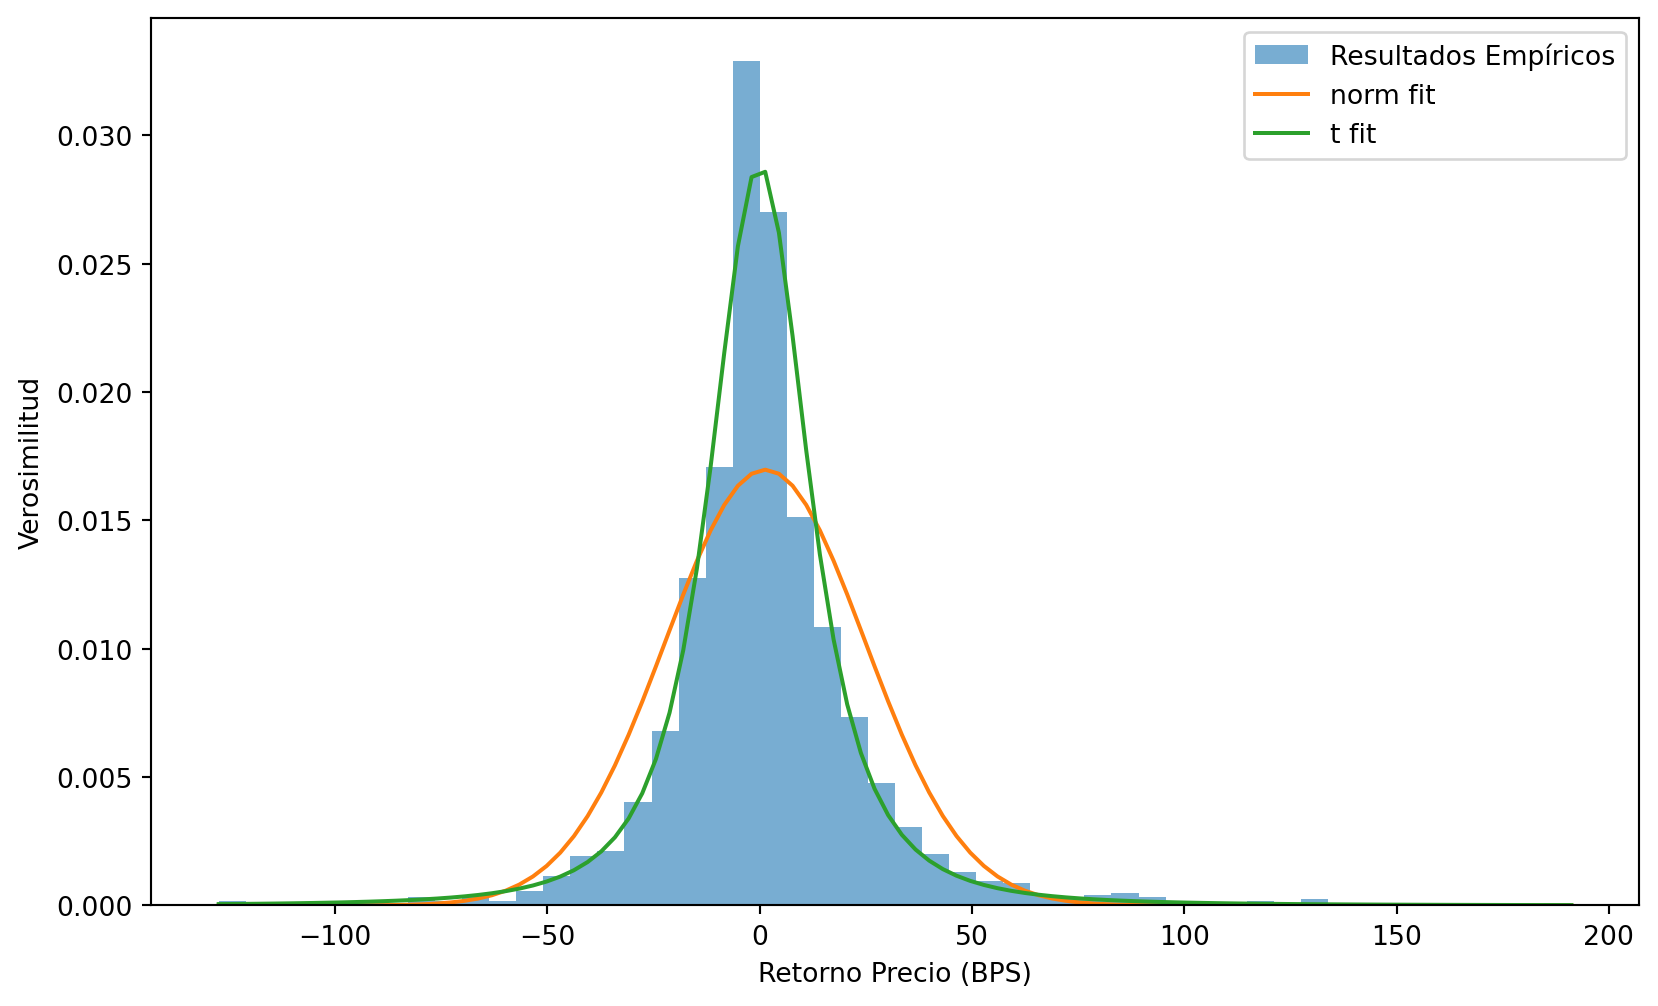
\includegraphics{index_files/figure-latex/notebooks-data-screening-fig-distribution-fitting-output-1.png}

}

\caption{\label{fig-distribution-fitting}Ajuste de distribuciones a los
retornos de precio.}

\end{figure}%

\textsubscript{Source:
\href{https://iancont.github.io/fixed_income_garch/index.qmd.html}{Article
Notebook}}

Al ajustar diferentes distribuciones a los retornos, observamos que la
distribución empírica (en azul) tiene una alta concentración en torno a
cero, con colas más gruesas de lo que se esperaría bajo una distribución
normal. Entre las distribuciones probadas, la t de Student (en rojo) es
la que mejor captura los valores extremos, con colas más largas y una
mayor concentración en el centro, lo que es típico en series financieras
que experimentan episodios de alta volatilidad. En contraste, la
distribución normal (en naranja) y la lognormal (en verde) subestiman
las colas, demostrando su ineficacia para modelar adecuadamente los
valores atípicos. Esto refuerza la idea de que la t de Student es una
mejor candidata para modelar los retornos, dado que puede ajustarse
mejor a la leptocurtosis observada en los datos.

\begin{figure}[H]

\centering{

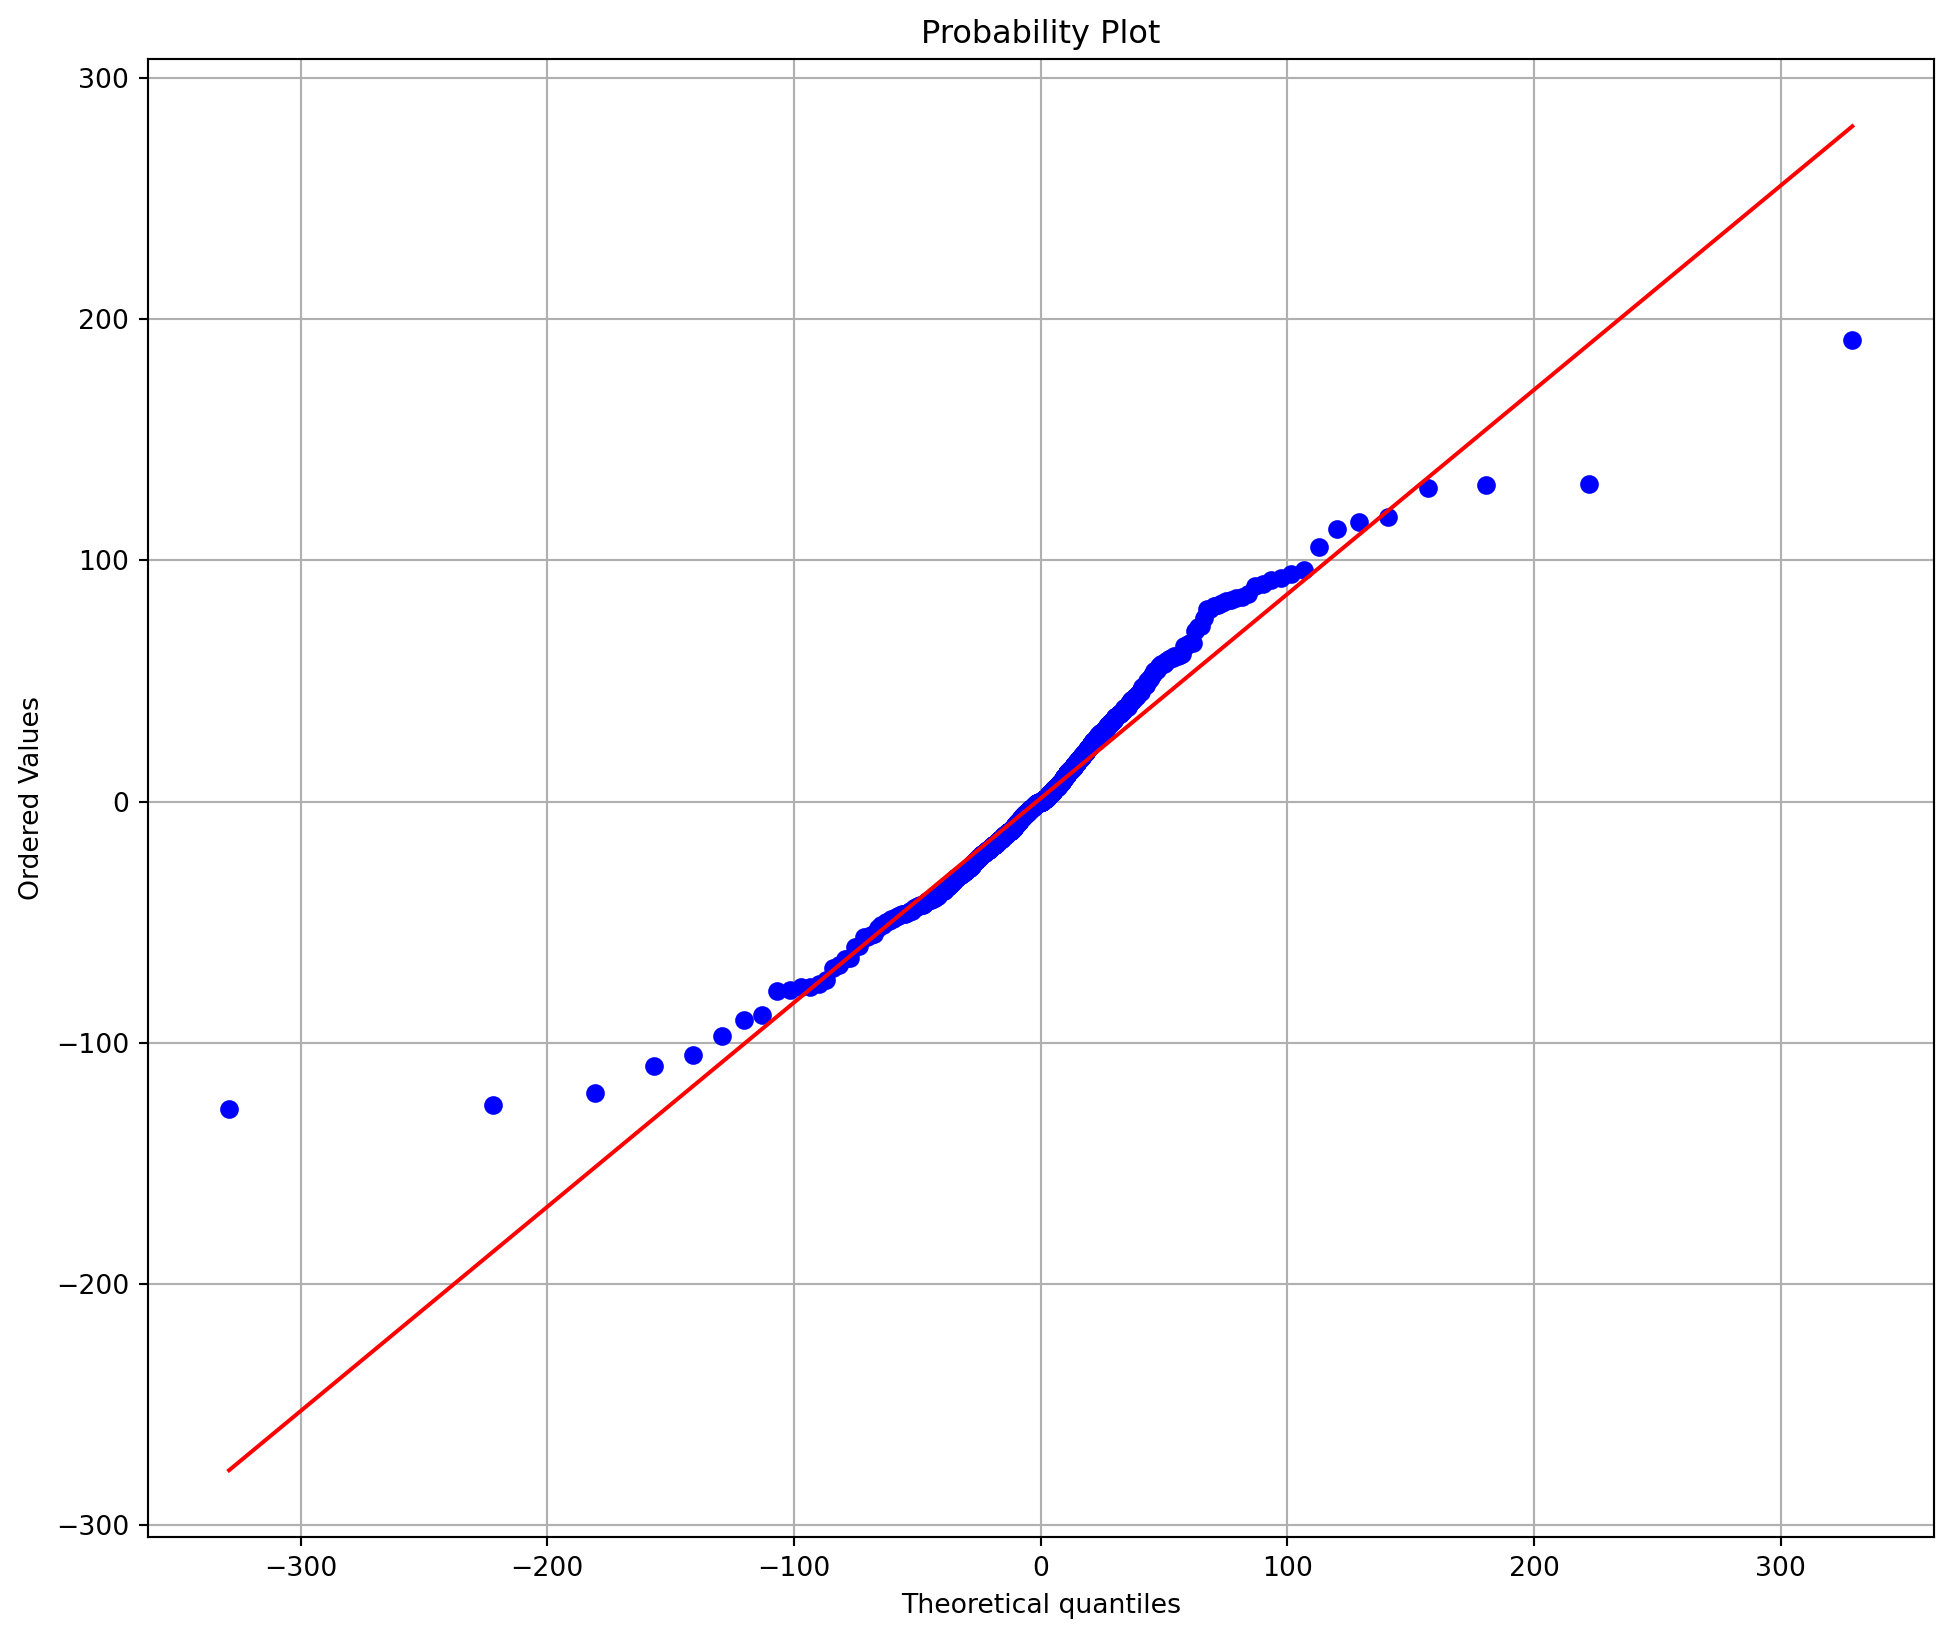
\includegraphics{index_files/figure-latex/notebooks-data-screening-fig-tqq-plot-output-1.png}

}

\caption{\label{fig-tqq-plot}Q-Q Plot de retornos de precio contra la
distribución t.}

\end{figure}%

\textsubscript{Source:
\href{https://iancont.github.io/fixed_income_garch/index.qmd.html}{Article
Notebook}}

La gráfica Q-Q (Quantile-Quantile) compara los cuantiles teóricos de la
distribución t de Student con los cuantiles observados de los retornos
del GOBIX. En general, la mayoría de los puntos se alinean bien con la
línea roja, lo que sugiere que los retornos de precios siguen
razonablemente esta distribución, particularmente en las partes
centrales. Sin embargo, en las colas extremas, se observan algunas
desviaciones, lo que indica que, aunque la t de Student es un buen
ajuste, no es perfecta para todos los escenarios.

El \textbf{estadístico de Kolmogorov-Smirnov} es de \(0.0286\), con un
\textbf{p-valor} de \(0.0827\). Aunque esto sugiere que la t de Student
captura bien la mayor parte de los retornos, las discrepancias en las
colas extremas muestran que la distribución teórica no es un ajuste
exacto a los datos reales.

\subsection{Evaluación de supuestos para análisis
AR-GARCH}\label{evaluaciuxf3n-de-supuestos-para-anuxe1lisis-ar-garch}

\subsubsection{Test de estacionariedad}\label{sec-estacionariedad}

Para garantizar la validez de los modelos ARMA y GARCH, se evaluó la
estacionariedad de la serie de retornos utilizando el test de
Dickey-Fuller aumentado (ADF). Los resultados obtenidos muestran un
\textbf{ADF Statistic} de \(-13.1741\) y un \textbf{p-valor} de
\(1.2333 \times 10^{-24}\), lo que permite rechazar la hipótesis nula de
raíz unitaria con un nivel de significancia del 5\%. Esto confirma que
la serie es estacionaria, lo que significa que sus fluctuaciones se
distribuyen alrededor de una media constante en el tiempo, sin tendencia
significativa. Este hallazgo es consistente con el comportamiento típico
de las series de retornos financieros, lo que habilita la correcta
estimación de modelos ARMA-GARCH para capturar las dinámicas del
mercado.

\subsubsection{Test de autocorrelación}\label{sec-autocorrelacion}

\begin{figure}[H]

\centering{

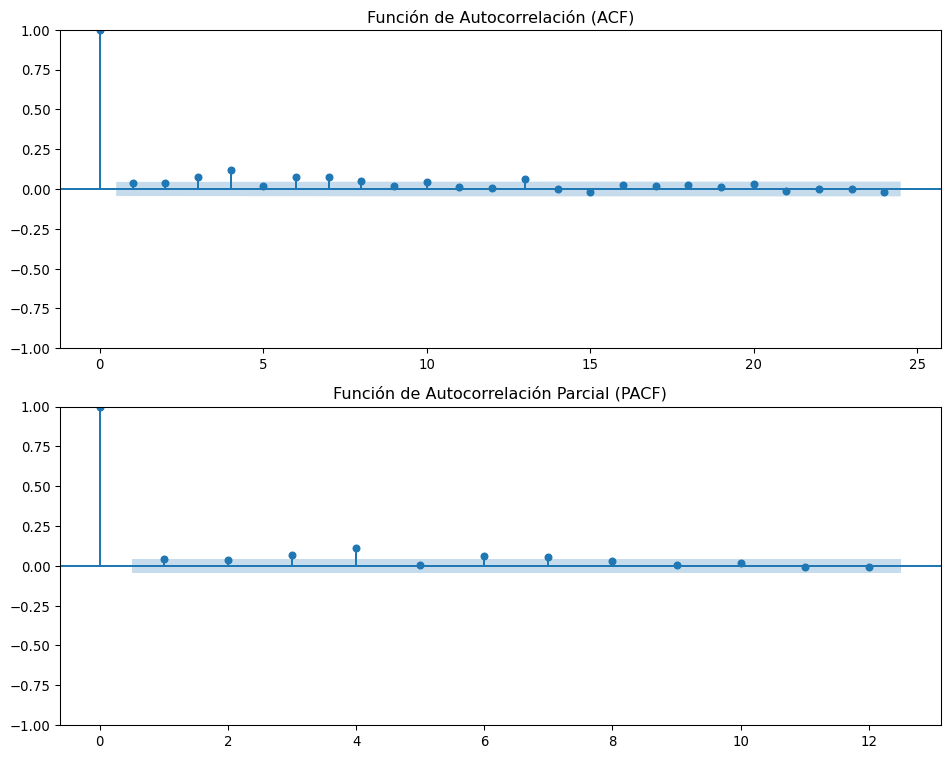
\includegraphics{index_files/figure-latex/notebooks-data-screening-fig-acf-pacf-output-1.png}

}

\caption{\label{fig-acf-pacf}Función de autocorrelación (ACF) y función
de autocorrelación parcial (PACF) de los retornos.}

\end{figure}%

\textsubscript{Source:
\href{https://iancont.github.io/fixed_income_garch/index.qmd.html}{Article
Notebook}}

El análisis de autocorrelación nos proporciona más detalles sobre la
estructura interna de la serie. El gráfico de la \textbf{Función de
Autocorrelación (ACF)} muestra un pico significativo en el primer
rezago, seguido de valores cercanos a cero para los rezagos posteriores.
Este patrón es indicativo de un proceso de media móvil de primer orden
(\textbf{MA(1)}), donde los choques aleatorios tienen un impacto
significativo en el primer rezago pero no en los siguientes. La
\textbf{Función de Autocorrelación Parcial (PACF)} refuerza esta
conclusión, mostrando un comportamiento similar con un pico en el primer
rezago y valores prácticamente nulos a partir del segundo rezago. Esto
sugiere que un modelo MA(1) sería apropiado para capturar las dinámicas
de corto plazo en la serie.

En conjunto, este análisis exploratorio sugiere que la serie de retornos
del IRP-GOBIX presenta características complejas, como
\textbf{volatility clustering}, alta \textbf{leptocurtosis}, y una
estructura de autocorrelación que se ajusta bien a un modelo MA(1).
Estos hallazgos proporcionan una base sólida para la estimación de
modelos ARMA-GARCH, los cuales podrán capturar de manera efectiva las
dinámicas de volatilidad y retornos en el mercado de deuda pública
dominicano.

\section{Resultados}\label{resultados}

El presente análisis tiene como objetivo modelar la serie temporal de
retornos del índice IRP-GOBIX utilizando inicialmente un modelo ARIMA
automático (auto-ARIMA) para determinar si es posible capturar la
dinámica de los retornos con un modelo basado únicamente en niveles y
diferencias de los datos. Adicionalmente, se evaluará la presencia de
problemas estructurales, como la heterocedasticidad, que podrían afectar
la consistencia del modelo ARIMA. En caso de que este enfoque no sea
adecuado, recurriremos a un modelo Zero-GARCH, un tipo específico de
GARCH que asume una media cero para los retornos. Este modelo es
particularmente útil en mercados de tasas de interés, donde se ha
demostrado que los retornos tienden a cero en el largo plazo debido a la
fuerte regresión hacia la media de estas variables.

\subsection{Análisis del modelo
ARIMA}\label{anuxe1lisis-del-modelo-arima}

\textsubscript{Source:
\href{https://iancont.github.io/fixed_income_garch/index.qmd.html}{Article
Notebook}}

\begin{center}
\begin{tabular}{lclc}
\toprule
\textbf{Dep. Variable:}          &        y         & \textbf{  No. Observations:  } &    1941     \\
\textbf{Model:}                  & SARIMAX(3, 0, 4) & \textbf{  Log Likelihood     } & -8853.517   \\
\textbf{Date:}                   & Sat, 19 Oct 2024 & \textbf{  AIC                } & 17725.034   \\
\textbf{Time:}                   &     15:47:38     & \textbf{  BIC                } & 17775.173   \\
\textbf{Sample:}                 &        0         & \textbf{  HQIC               } & 17743.472   \\
\textbf{}                        &      - 1941      & \textbf{                     } &             \\
\textbf{Covariance Type:}        &       opg        & \textbf{                     } &             \\
\bottomrule
\end{tabular}
\begin{tabular}{lcccccc}
                   & \textbf{coef} & \textbf{std err} & \textbf{z} & \textbf{P$> |$z$|$} & \textbf{[0.025} & \textbf{0.975]}  \\
\midrule
\textbf{intercept} &       0.3602  &        0.273     &     1.317  &         0.188        &       -0.176    &        0.896     \\
\textbf{ar.L1}     &       0.1366  &        0.065     &     2.106  &         0.035        &        0.009    &        0.264     \\
\textbf{ar.L2}     &      -0.1931  &        0.066     &    -2.934  &         0.003        &       -0.322    &       -0.064     \\
\textbf{ar.L3}     &       0.7691  &        0.061     &    12.644  &         0.000        &        0.650    &        0.888     \\
\textbf{ma.L1}     &      -0.1139  &        0.065     &    -1.752  &         0.080        &       -0.241    &        0.014     \\
\textbf{ma.L2}     &       0.2163  &        0.067     &     3.220  &         0.001        &        0.085    &        0.348     \\
\textbf{ma.L3}     &      -0.7032  &        0.062     &   -11.315  &         0.000        &       -0.825    &       -0.581     \\
\textbf{ma.L4}     &       0.0750  &        0.020     &     3.715  &         0.000        &        0.035    &        0.115     \\
\textbf{sigma2}    &     536.2183  &        8.358     &    64.154  &         0.000        &      519.836    &      552.600     \\
\bottomrule
\end{tabular}
\begin{tabular}{lclc}
\textbf{Ljung-Box (L1) (Q):}     & 0.00 & \textbf{  Jarque-Bera (JB):  } & 4395.18  \\
\textbf{Prob(Q):}                & 1.00 & \textbf{  Prob(JB):          } &   0.00   \\
\textbf{Heteroskedasticity (H):} & 1.11 & \textbf{  Skew:              } &   0.59   \\
\textbf{Prob(H) (two-sided):}    & 0.17 & \textbf{  Kurtosis:          } &  10.28   \\
\bottomrule
\end{tabular}
%\caption{SARIMAX Results}
\end{center}

Warnings: \newline
 [1] Covariance matrix calculated using the outer product of gradients (complex-step).

Modelo ARIMA de maxima verosimilitud para la serie de retornos.

\textsubscript{Source:
\href{https://iancont.github.io/fixed_income_garch/index.qmd.html}{Article
Notebook}}

El modelo SARIMAX(3, 0, 4) se estimó con el objetivo de capturar la
dinámica subyacente de la serie de retornos. Aunque los resultados
muestran que algunos de los coeficientes del componente autorregresivo
(AR) y del promedio móvil (MA) son estadísticamente significativos
(e.g., \(AR(3)\) con un coeficiente de \(0.7691\), \(p < 0.001\) y
\(MA(2)\) con \(p < 0.01\)), el desempeño general del modelo presenta
ciertas limitaciones. El test de heterocedasticidad muestra un valor de
1.11, lo que indica la presencia de heterocedasticidad en la serie, un
problema común en series financieras, donde la varianza de los errores
no es constante a lo largo del tiempo.

Además, el estadístico de Jarque-Bera de 4395.18, con una probabilidad
de \(p = 0.00\), confirma que los residuos no siguen una distribución
normal, lo que refuerza la idea de que un modelo basado únicamente en
niveles, como el ARIMA, podría no ser suficiente para capturar la
volatilidad inherente a los retornos del mercado de deuda pública
dominicano. Dado que los modelos ARIMA no están diseñados para abordar
adecuadamente la heterocedasticidad, pasamos a estimar un modelo GARCH,
que es más apropiado para capturar los cambios en la volatilidad.

\subsection{Modelo Zero-GARCH}\label{modelo-zero-garch}

Para abordar las limitaciones del modelo ARIMA, se estimó un modelo
GARCH(1,1) con media cero, siguiendo la estructura propuesta por
\citep{miah_rahman_2016}, quienes demostrarón que los modelos GARCH(1,1)
son altamente efectivos para capturar la volatilidad en los retornos de
mercados financieros. La elección de un modelo con media cero se
justifica porque en mercados de deuda pública y tasas de interés, los
retornos tienden a revertir a la media, y en el largo plazo se espera
que los retornos por apreciación de capital converjan a cero.
\citep{fabozzi_fixed_income}

\textsubscript{Source:
\href{https://iancont.github.io/fixed_income_garch/index.qmd.html}{Article
Notebook}}

\phantomsection\label{garch-model-fitting}
\textsubscript{Source:
\href{https://iancont.github.io/fixed_income_garch/index.qmd.html}{Article
Notebook}}

\begin{center}
\begin{tabular}{lclc}
\toprule
\textbf{Dep. Variable:} &      price\_return       & \textbf{  R-squared:         } &     0.000   \\
\textbf{Mean Model:}    &        Zero Mean         & \textbf{  Adj. R-squared:    } &     0.001   \\
\textbf{Vol Model:}     &          GARCH           & \textbf{  Log-Likelihood:    } &   -7622.87  \\
\textbf{Distribution:}  & Standardized Student's t & \textbf{  AIC:               } &    15253.7  \\
\textbf{Method:}        &    Maximum Likelihood    & \textbf{  BIC:               } &    15275.6  \\
\textbf{}               &                          & \textbf{  No. Observations:  } &    1753     \\
\textbf{Date:}          &     Sat, Oct 19 2024     & \textbf{  Df Residuals:      } &    1753     \\
\textbf{Time:}          &         15:47:38         & \textbf{  Df Model:          } &     0       \\
\bottomrule
\end{tabular}
\begin{tabular}{lccccc}
                  & \textbf{coef} & \textbf{std err} & \textbf{t} & \textbf{P$> |$t$|$} & \textbf{95.0\% Conf. Int.}  \\
\midrule
\textbf{omega}    &      58.8679  &       25.182     &     2.338  &      1.940e-02       &    [  9.512,1.082e+02]      \\
\textbf{alpha[1]} &       0.1892  &    6.657e-02     &     2.842  &      4.482e-03       &    [5.873e-02,  0.320]      \\
\textbf{beta[1]}  &       0.7737  &    6.832e-02     &    11.324  &      9.943e-30       &     [  0.640,  0.908]       \\
            & \textbf{coef} & \textbf{std err} & \textbf{t} & \textbf{P$> |$t$|$} & \textbf{95.0\% Conf. Int.}  \\
\midrule
\textbf{nu} &       2.7894  &        0.230     &    12.114  &      8.853e-34       &     [  2.338,  3.241]       \\
\bottomrule
\end{tabular}
%\caption{Zero Mean - GARCH Model Results}
\end{center}

Covariance estimator: robust

Modelo Zero-Garch de la serie de retornos

\textsubscript{Source:
\href{https://iancont.github.io/fixed_income_garch/index.qmd.html}{Article
Notebook}}

Los resultados del modelo Zero-GARCH confirman un buen ajuste a la
volatilidad de la serie de retornos. El coeficiente \(\omega\) del
proceso de volatilidad es de \(58.8679\) (\(p < 0.05\)), lo que indica
un nivel base significativo de volatilidad en la serie. El parámetro
\(\alpha_1\), que mide la influencia de los shocks pasados en la
volatilidad actual, es positivo y significativo (\(0.1892\),
\(p < 0.01\)), lo que sugiere que los shocks pasados tienen un impacto
considerable en la volatilidad presente. Por otro lado, \(\beta_1\)
(\(0.7737\), \(p < 0.001\)) indica que existe una fuerte persistencia en
la volatilidad, característica común en los mercados financieros, donde
las fases de alta volatilidad tienden a durar varios periodos.

El uso de la distribución t de Student para los residuos estandarizados,
con un parámetro \(\nu\) de \(2.7894\) (\(p < 0.001\)), confirma la
presencia de colas más gruesas en la distribución de los retornos, lo
que es consistente con la leptocurtosis observada en la serie de
retornos.

\subsubsection{Residuos del Zero-GARCH}\label{residuos-del-zero-garch}

\begin{figure}[H]

\centering{

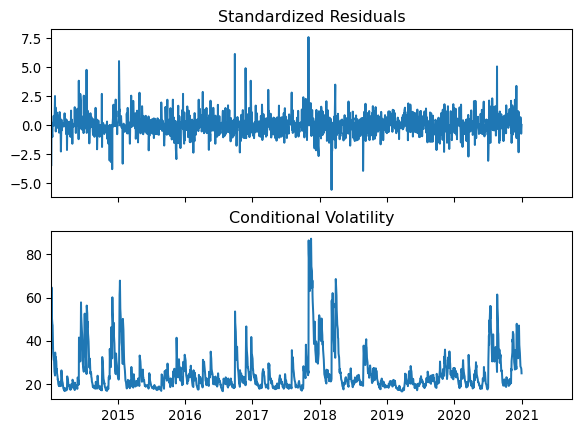
\includegraphics{index_files/figure-latex/notebooks-data-screening-fig-garch-residuals-output-1.png}

}

\caption{\label{fig-garch-residuals}Residuos del modelo AR-GARCH.}

\end{figure}%

\textsubscript{Source:
\href{https://iancont.github.io/fixed_income_garch/index.qmd.html}{Article
Notebook}}

Al analizar los residuos estandarizados y la volatilidad condicional en
el modelo Zero-GARCH, observamos cómo la volatilidad responde de manera
dinámica a los choques en los retornos. En la primera gráfica, se
aprecia que la volatilidad condicional es mayor durante episodios donde
los residuos estandarizados alcanzan picos extremos, especialmente en
periodos de alta volatilidad como 2018. Esto refuerza la capacidad del
modelo GARCH para capturar \textbf{volatility clustering}, un fenómeno
donde la alta volatilidad tiende a agruparse en ciertos periodos.
Además, la persistencia de la volatilidad condicional a lo largo del
tiempo confirma que los choques pasados tienen un efecto prolongado, lo
cual es coherente con los resultados obtenidos en los coeficientes del
modelo GARCH.

\subsubsection{Residuos contra volatilidad
condicional}\label{residuos-contra-volatilidad-condicional}

\begin{figure}[H]

\centering{

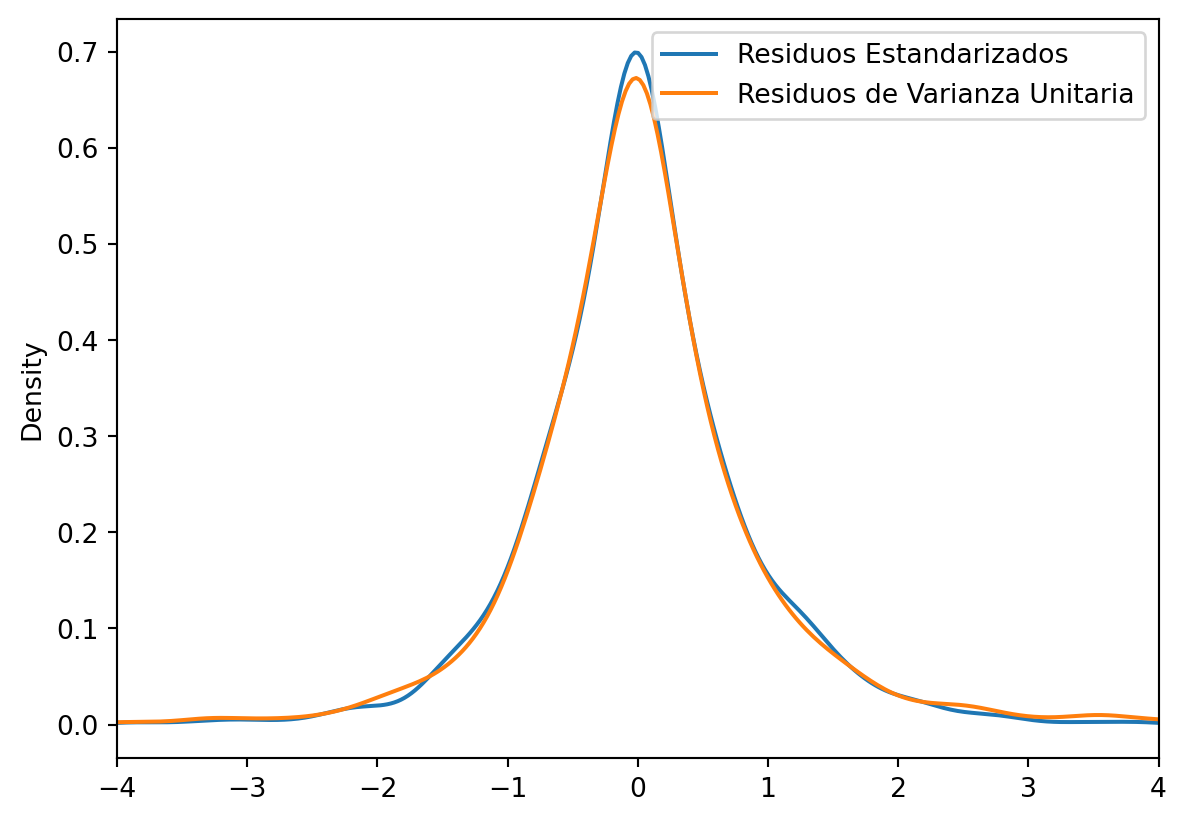
\includegraphics{index_files/figure-latex/notebooks-data-screening-fig-residuals-vs-volatility-output-1.png}

}

\caption{\label{fig-residuals-vs-volatility}Residuos contra la
volatilidad condicional del AR-GARCH.}

\end{figure}%

\textsubscript{Source:
\href{https://iancont.github.io/fixed_income_garch/index.qmd.html}{Article
Notebook}}

En cuanto a la comparación entre los residuos estandarizados y los
residuos de varianza unitaria, la segunda gráfica revela que ambos
conjuntos de residuos presentan distribuciones similares, con una alta
concentración alrededor de cero. Sin embargo, las colas más gruesas en
los residuos estandarizados indican la presencia de eventos extremos más
pronunciados, los cuales son típicos en series financieras que presentan
leptocurtosis. Esta comparación subraya la importancia de utilizar
distribuciones robustas, como la t de Student, para capturar
adecuadamente las colas de la distribución, tal como lo hace el modelo
GARCH en este caso.

Los resultados del modelo Zero-GARCH confirman su capacidad para modelar
de manera efectiva la volatilidad en los retornos del IRP-GOBIX. Aunque
el modelo auto-ARIMA capturó algunos patrones de la serie, su
inconsistencia en la presencia de heterocedasticidad subraya la
necesidad de un enfoque basado en modelos GARCH. El modelo Zero-GARCH no
solo demuestra un buen ajuste a los datos, sino que también captura la
dinámica de la volatilidad condicional y los residuos estandarizados,
revelando la presencia de \textbf{volatility clustering} y la
persistencia en la volatilidad.

La comparación entre los residuos estandarizados y los residuos de
varianza unitaria destaca la capacidad del modelo para manejar eventos
extremos, una característica esencial en el análisis de series
financieras. En resumen, el modelo Zero-GARCH es más robusto y adecuado
para describir las dinámicas de volatilidad en el mercado de deuda
pública dominicano, brindando información crucial sobre la persistencia
y el comportamiento de la volatilidad a lo largo del tiempo.

\subsection{Evaluación Retrospectiva
(Backtesting)}\label{evaluaciuxf3n-retrospectiva-backtesting}

Para evaluar la capacidad predictiva del modelo Zero-GARCH, se realizó
un análisis de backtesting sobre el periodo comprendido durante el año
2021. Se emplearon dos métodos principales de evaluación: el MAPE (Mean
Absolute Percentage Error) y el análisis gráfico de los valores
predichos frente a los valores actuales de la desviación estándar móvil.

\begin{figure}[H]

\centering{

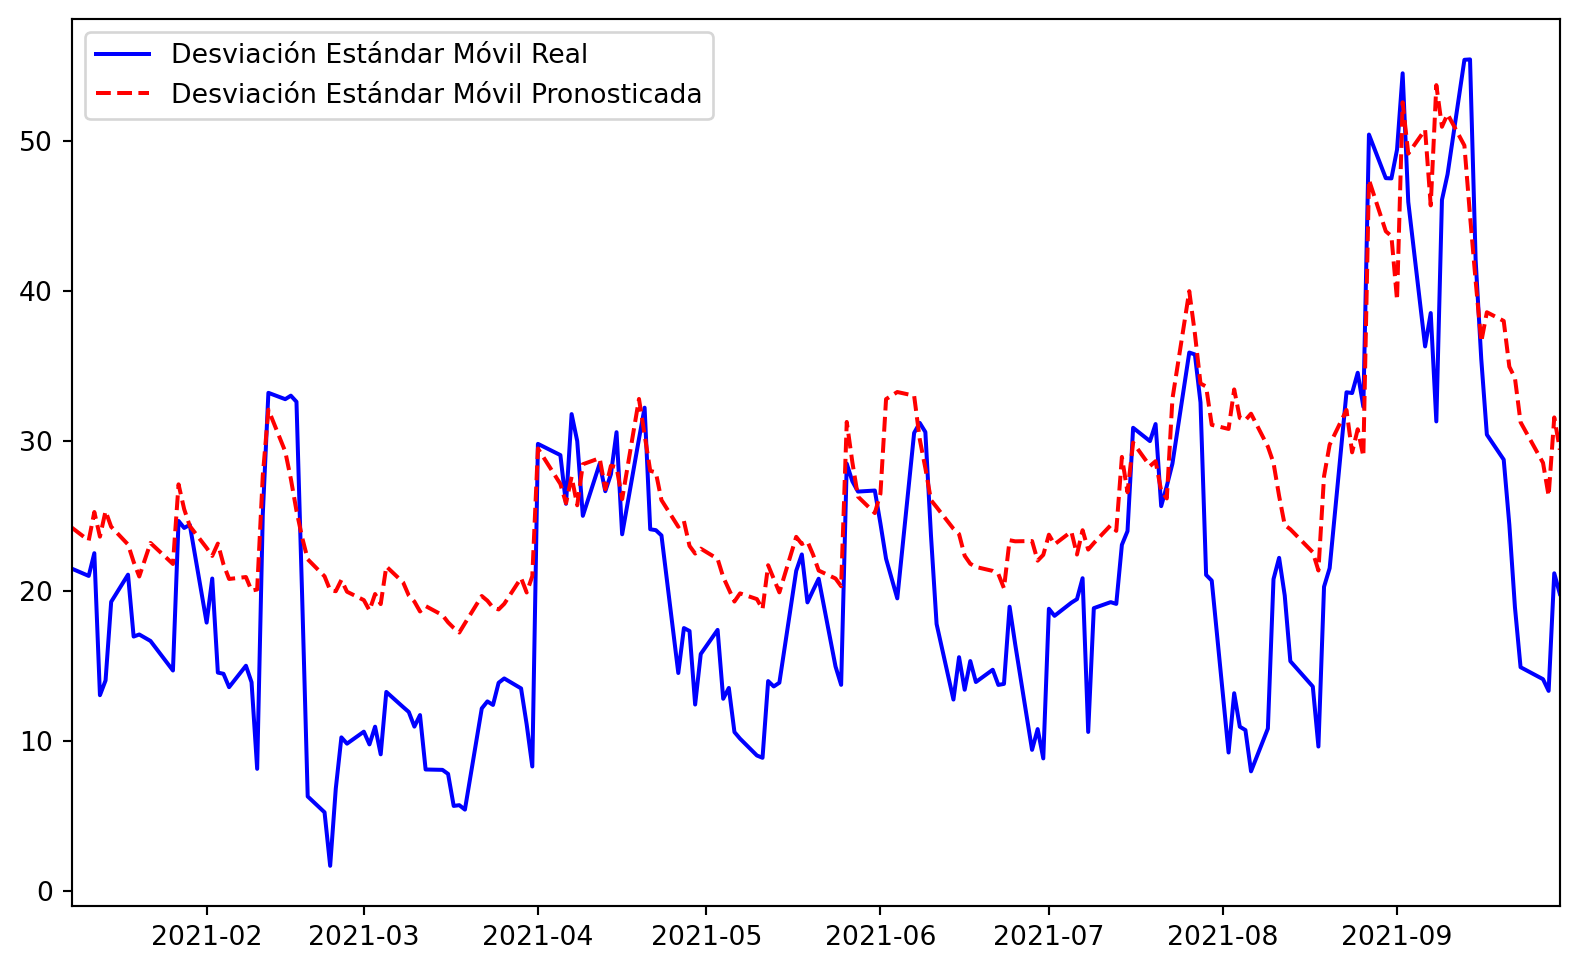
\includegraphics{index_files/figure-latex/notebooks-data-screening-fig-predicted-vs-actual-backtest-output-1.png}

}

\caption{\label{fig-predicted-vs-actual-backtest}Desviación Estándar
Móvil Real vs Pronosticada - Modelo Zero-GARCH}

\end{figure}%

\textsubscript{Source:
\href{https://iancont.github.io/fixed_income_garch/index.qmd.html}{Article
Notebook}}

El análisis gráfico (Predichos vs Actuales) revela que el modelo captura
de manera excelente la \textbf{tendencia} general de la serie, lo que
implica que el modelo es eficiente a la hora de predecir los movimientos
de largo plazo en la volatilidad. Sin embargo, un problema importante
que surge es que el modelo tiende a suavizar los movimientos bruscos,
especialmente en momentos donde la volatilidad sufre caídas o picos
repentinos. Este fenómeno de \textbf{sobre-suavización} implica que el
modelo no es completamente reactivo a los choques regresivos de gran
magnitud, lo que puede deberse a la estructura propia del GARCH, la cual
tiende a modelar la volatilidad alrededor de la media del periodo.

El MAPE calculado para el conjunto de test arroja un valor elevado de
\textbf{739.70\%}, lo cual podría sugerir en un análisis superficial que
el modelo no es adecuado. Sin embargo, es importante considerar el tipo
de mercado con el que estamos trabajando, caracterizado por una
volatilidad intrínsecamente elevada y movimientos extremos. En estos
contextos, valores altos de MAPE son comunes debido a la alta
variabilidad en los retornos, lo que no necesariamente implica una mala
capacidad predictiva, sino que refleja la naturaleza errática de los
datos financieros. En este sentido, el MAPE alto está más relacionado
con la complejidad del mercado que con la falta de ajuste del modelo.

El backtesting del modelo Zero-GARCH sobre la serie de retornos del
IRP-GOBIX para el periodo de 2021 confirma que, si bien el modelo
captura correctamente la tendencia general de la volatilidad, su
capacidad para reaccionar ante movimientos abruptos es limitada. A pesar
de esto, dado el contexto del mercado de deuda pública dominicano, la
sobre-suavización en los niveles es un comportamiento esperado en
modelos de volatilidad como el GARCH. En resumen, el modelo es útil para
predecir tendencias a largo plazo, pero su precisión en niveles podría
mejorarse si se ajusta para reaccionar mejor a eventos extremos.

\section{Discusión y Conclusión}\label{discusiuxf3n-y-conclusiuxf3n}

\subsection{Discusión}\label{discusiuxf3n}

Este estudio ha permitido modelar los retornos y la volatilidad del
mercado de deuda pública dominicano utilizando modelos ARIMA-GARCH. A
pesar de los hallazgos significativos, existen algunas limitaciones que
deben considerarse al interpretar los resultados:

\begin{itemize}
\item
  \textbf{Problemas con la sobre-suavización}: Como se observó en el
  análisis retrospectivo, el modelo Zero-GARCH tiende a suavizar los
  movimientos bruscos en la volatilidad, lo que puede limitar su
  capacidad de capturar adecuadamente choques repentinos en el mercado.
  Aunque el modelo refleja bien la tendencia general, su capacidad de
  reacción frente a eventos extremos debe ser mejorada.
\item
  \textbf{MAPE elevado}: El MAPE obtenido durante la evaluación
  retrospectiva fue considerablemente alto. Si bien esto puede
  justificarse por la naturaleza volátil del mercado de deuda pública,
  sugiere que el modelo puede tener problemas para ajustarse a los
  movimientos de corto plazo. La alta volatilidad y los choques
  repentinos no fueron capturados con precisión, afectando el
  rendimiento del modelo.
\item
  \textbf{Limitaciones en los datos}: El análisis se centró en un
  período específico (2014-2021), excluyendo la pandemia debido a sus
  características atípicas. Si bien esto ayudó a evitar sesgos, la
  exclusión de este período crítico puede haber omitido dinámicas
  importantes del mercado en tiempos de crisis, limitando la
  generalización de los resultados.
\end{itemize}

\subsection{Conclusión}\label{conclusiuxf3n}

En conclusión, este estudio ha demostrado que el modelo ARIMA, aunque
útil para capturar la estructura de los retornos del mercado de deuda
pública dominicano, presenta limitaciones cuando se enfrenta a problemas
de heterocedasticidad. El modelo Zero-GARCH, por su parte, ha demostrado
ser más adecuado para describir la dinámica de la volatilidad,
capturando fenómenos como la persistencia en la volatilidad y el
clustering. Además, la capacidad del modelo para manejar eventos
extremos a través de la distribución t de Student resulta valiosa en
este tipo de mercados caracterizados por alta volatilidad y choques
inesperados.

Entre los principales hallazgos destacan:

\begin{itemize}
\item
  \textbf{Volatility clustering}: El análisis confirmó la presencia de
  agrupación de volatilidad, donde periodos de baja volatilidad son
  seguidos por periodos de alta volatilidad, un fenómeno común en los
  mercados financieros.
\item
  \textbf{Persistencia de la volatilidad}: El coeficiente \(\beta_1\)
  significativo en el modelo GARCH sugiere que los shocks en la
  volatilidad tienen un efecto prolongado en el tiempo, lo que es
  consistente con los patrones observados en mercados financieros
  emergentes como el dominicano.
\item
  \textbf{Dificultad para capturar movimientos extremos}: Aunque el
  modelo Zero-GARCH es efectivo en capturar la tendencia general, su
  capacidad para reaccionar ante cambios bruscos en la volatilidad sigue
  siendo limitada, lo cual es un área de mejora para futuras
  investigaciones.
\item
  \textbf{Implicaciones para los inversores}: Los resultados ofrecen una
  herramienta útil para la predicción de tendencias de volatilidad a
  largo plazo en el mercado de deuda pública dominicano, proporcionando
  una base para la toma de decisiones estratégicas en la gestión del
  riesgo.
\end{itemize}

Este estudio no solo contribuye al entendimiento del comportamiento de
los retornos y la volatilidad en el mercado de deuda pública dominicano.

\section{Referencias}\label{referencias}

\textsubscript{Source:
\href{https://iancont.github.io/fixed_income_garch/index.qmd.html}{Article
Notebook}}


  \bibliography{references.bib}



\end{document}
